\documentclass[journal,12pt,twocolumn]{IEEEtran}
%
\usepackage{setspace}
\usepackage{gensymb}
%\doublespacing
\singlespacing

%\usepackage{graphicx}
%\usepackage{amssymb}
%\usepackage{relsize}
\usepackage[cmex10]{amsmath}
%\usepackage{amsthm}
%\interdisplaylinepenalty=2500
%\savesymbol{iint}
%\usepackage{txfonts}
%\restoresymbol{TXF}{iint}
%\usepackage{wasysym}
\usepackage{amsthm}
%\usepackage{iithtlc}
\usepackage{mathrsfs}
\usepackage{txfonts}
\usepackage{stfloats}
\usepackage{bm}
\usepackage{cite}
\usepackage{cases}
\usepackage{subfig}
%\usepackage{xtab}
\usepackage{longtable}
\usepackage{multirow}
%\usepackage{algorithm}
%\usepackage{algpseudocode}
\usepackage{enumitem}
\usepackage{mathtools}
\usepackage{steinmetz}
\usepackage{tikz}
\usepackage{circuitikz}
\usepackage{verbatim}
\usepackage{tfrupee}
\usepackage[breaklinks=true]{hyperref}
%\usepackage{stmaryrd}
\usepackage{tkz-euclide} % loads  TikZ and tkz-base
%\usetkzobj{all}
\usetikzlibrary{calc,math}
\usepackage{listings}
    \usepackage{color}                                            %%
    \usepackage{array}                                            %%
    \usepackage{longtable}                                        %%
    \usepackage{calc}                                             %%
    \usepackage{multirow}                                         %%
    \usepackage{hhline}                                           %%
    \usepackage{ifthen}                                           %%
  %optionally (for landscape tables embedded in another document): %%
    \usepackage{lscape}     
\usepackage{multicol}
\usepackage{chngcntr}
%\usepackage{enumerate}

%\usepackage{wasysym}
%\newcounter{MYtempeqncnt}
\DeclareMathOperator*{\Res}{Res}
%\renewcommand{\baselinestretch}{2}
\renewcommand\thesection{\arabic{section}}
\renewcommand\thesubsection{\thesection.\arabic{subsection}}
\renewcommand\thesubsubsection{\thesubsection.\arabic{subsubsection}}

\renewcommand\thesectiondis{\arabic{section}}
\renewcommand\thesubsectiondis{\thesectiondis.\arabic{subsection}}
\renewcommand\thesubsubsectiondis{\thesubsectiondis.\arabic{subsubsection}}

% correct bad hyphenation here
\hyphenation{op-tical net-works semi-conduc-tor}
\def\inputGnumericTable{}                                 %%

\lstset{
%language=C,
frame=single, 
breaklines=true,
columns=fullflexible
}
%\lstset{
%language=tex,
%frame=single, 
%breaklines=true
%}

\begin{document}
%


\newtheorem{theorem}{Theorem}[section]
\newtheorem{problem}{Problem}
\newtheorem{proposition}{Proposition}[section]
\newtheorem{lemma}{Lemma}[section]
\newtheorem{corollary}[theorem]{Corollary}
\newtheorem{example}{Example}[section]
\newtheorem{definition}[problem]{Definition}
%\newtheorem{thm}{Theorem}[section] 
%\newtheorem{defn}[thm]{Definition}
%\newtheorem{algorithm}{Algorithm}[section]
%\newtheorem{cor}{Corollary}
\newcommand{\BEQA}{\begin{eqnarray}}
\newcommand{\EEQA}{\end{eqnarray}}
\newcommand{\define}{\stackrel{\triangle}{=}}

\bibliographystyle{IEEEtran}
%\bibliographystyle{ieeetr}


\providecommand{\mbf}{\mathbf}
\providecommand{\pr}[1]{\ensuremath{\Pr\left(#1\right)}}
\providecommand{\qfunc}[1]{\ensuremath{Q\left(#1\right)}}
\providecommand{\sbrak}[1]{\ensuremath{{}\left[#1\right]}}
\providecommand{\lsbrak}[1]{\ensuremath{{}\left[#1\right.}}
\providecommand{\rsbrak}[1]{\ensuremath{{}\left.#1\right]}}
\providecommand{\brak}[1]{\ensuremath{\left(#1\right)}}
\providecommand{\lbrak}[1]{\ensuremath{\left(#1\right.}}
\providecommand{\rbrak}[1]{\ensuremath{\left.#1\right)}}
\providecommand{\cbrak}[1]{\ensuremath{\left\{#1\right\}}}
\providecommand{\lcbrak}[1]{\ensuremath{\left\{#1\right.}}
\providecommand{\rcbrak}[1]{\ensuremath{\left.#1\right\}}}
\theoremstyle{remark}
\newtheorem{rem}{Remark}
\newcommand{\sgn}{\mathop{\mathrm{sgn}}}
\providecommand{\abs}[1]{\left\vert#1\right\vert}
\providecommand{\res}[1]{\Res\displaylimits_{#1}} 
\providecommand{\norm}[1]{\left\lVert#1\right\rVert}
%\providecommand{\norm}[1]{\lVert#1\rVert}
\providecommand{\mtx}[1]{\mathbf{#1}}
\providecommand{\mean}[1]{E\left[ #1 \right]}
\providecommand{\fourier}{\overset{\mathcal{F}}{ \rightleftharpoons}}
%\providecommand{\hilbert}{\overset{\mathcal{H}}{ \rightleftharpoons}}
\providecommand{\system}{\overset{\mathcal{H}}{ \longleftrightarrow}}
	%\newcommand{\solution}[2]{\textbf{Solution:}{#1}}
\newcommand{\solution}{\noindent \textbf{Solution: }}
\newcommand{\cosec}{\,\text{cosec}\,}
\providecommand{\dec}[2]{\ensuremath{\overset{#1}{\underset{#2}{\gtrless}}}}
\newcommand{\myvec}[1]{\ensuremath{\begin{pmatrix}#1\end{pmatrix}}}
\newcommand{\mydet}[1]{\ensuremath{\begin{vmatrix}#1\end{vmatrix}}}
%\numberwithin{equation}{section}
\numberwithin{equation}{subsection}
%\numberwithin{problem}{section}
%\numberwithin{definition}{section}
\makeatletter
\@addtoreset{figure}{problem}
\makeatother

\let\StandardTheFigure\thefigure
\let\vec\mathbf
%\renewcommand{\thefigure}{\theproblem.\arabic{figure}}
\renewcommand{\thefigure}{\theproblem}
%\setlist[enumerate,1]{before=\renewcommand\theequation{\theenumi.\arabic{equation}}
%\counterwithin{equation}{enumi}


%\renewcommand{\theequation}{\arabic{subsection}.\arabic{equation}}

\def\putbox#1#2#3{\makebox[0in][l]{\makebox[#1][l]{}\raisebox{\baselineskip}[0in][0in]{\raisebox{#2}[0in][0in]{#3}}}}
     \def\rightbox#1{\makebox[0in][r]{#1}}
     \def\centbox#1{\makebox[0in]{#1}}
     \def\topbox#1{\raisebox{-\baselineskip}[0in][0in]{#1}}
     \def\midbox#1{\raisebox{-0.5\baselineskip}[0in][0in]{#1}}

\vspace{3cm}


\title{Assignment 6}
\author{Jayati Dutta}





% make the title area
\maketitle

\newpage

%\tableofcontents

\bigskip

\renewcommand{\thefigure}{\theenumi}
\renewcommand{\thetable}{\theenumi}
%\renewcommand{\theequation}{\theenumi}


\begin{abstract}
This is a simple document explaining how to determine a conic section from a given second degree equation.
\end{abstract}

%Download all python codes 
%
%\begin{lstlisting}
%svn co https://github.com/JayatiD93/trunk/My_solution_design/codes
%\end{lstlisting}

Download all and latex-tikz codes from 
%
\begin{lstlisting}
svn co https://github.com/gadepall/school/trunk/ncert/geometry/figs
\end{lstlisting}
%


\section{Problem}
What conics do the following equation represents? When possible, find the center and the equation reffered to the center.
\begin{multline}
55x^2 - 120xy + 20y^2 +64x -48y=0
\label{eqn1}
\end{multline}

\section{Explanation}
The general equation of second degree can be represented as:
\begin{align}
\vec{X}^T\vec{V}\vec{X} + 2\vec{u}^T\vec{X} + f = 0
\end{align}
The above \ref{eqn1} can also be written as:
\begin{align}
\vec{X}^T\myvec{55 & -60\\-60 & 20}\vec{X} + 2\myvec{32 & -24}\vec{X} +0 = 0
\end{align}
So, 
\begin{align}
\vec{V} = \myvec{55 & -60\\-60 & 20}
\end{align}
and 
\begin{align}
\vec{u} = \myvec{32 \\ -24}\\
f=0
\end{align}
Now, 
\begin{align}
\det{\vec{V}} = \mydet{55 & -60\\-60 & 20}\\
\implies \det{\vec{V}} = -2500 <0
\end{align}

As $\det{\vec{V}}<0$, so we can say that the above conic section \ref{eqn1} is hyperbola.Now,
\begin{align}
\vec{V}^{-1} =\frac{1}{-2500} \myvec{20 & 60\\60 & 55}
\end{align}
The center of this hyperbola will be:
\begin{align}
\vec{c} = - \vec{V}^{-1} \vec{u}\\
\implies \vec{c} = \frac{1}{2500} \myvec{20 & 60\\60 & 55} \myvec{32 \\ -24}\\
\implies \vec{c} = \myvec{-\frac{8}{25} \\ \frac{6}{25}}\\
\end{align}
 Now the characteristic equation of $\vec{V}$ is obtained as:
\begin{align}
\mydet{\vec{V} - \lambda\vec{I}} =0\\
\implies \mydet{55-\lambda & -60\\-60 & 20-\lambda} = 0\\
\implies \lambda^2 - 75\lambda - 2500=0
\end{align}
The eigen values are given by:
\begin{align}
\lambda_1=100\\
\lambda_2 = -25
\end{align}
The eigen vector $\vec{P}$ is defined as:
\begin{align}
\vec{V}\vec{P} = \lambda \vec{P}\\
\implies (\vec{V} -\lambda\vec{I})\vec{P} = \vec{0}
\end{align}
For $\lambda_1$=100,
\begin{align}
(\vec{V} -\lambda_1\vec{I}) = \myvec{-45 & -60\\-60 & -80}
\end{align}
By row reduction,
\begin{align}
\myvec{-45 & -60\\-60 & -80}\xleftrightarrow[R_1\leftarrow R_1 /(-5)]{R_2\leftarrow R_2/(-5)}\\
\myvec{9 & 12\\12 & 16}\xleftrightarrow[R_1\leftarrow R_1 /3]{R_2\leftarrow R_2/4}\\
\myvec{3 & 4\\3 & 4}\xleftrightarrow[]{R_2\leftarrow R_2-R_1}\myvec{3 & 4\\0 & 0}
\end{align}
So, 
\begin{align}
(\vec{V} -\lambda_1\vec{I})\vec{P_1} = \vec{0}\\
\implies \myvec{3 & 4\\0 & 0} \myvec{v_1\\v_2} = \myvec{0\\0}\\
\implies \vec{P_1} = \myvec{-\frac{4}{3}\\1}
\end{align}
Similarly,
For $\lambda_2$=100,
\begin{align}
(\vec{V} -\lambda_2\vec{I}) = \myvec{80 & -60\\-60 & 45}
\end{align}
By row reduction,
\begin{align}
\myvec{80 & -60\\-60 & 45}\xleftrightarrow[R_1\leftarrow R_1 /5]{R_2\leftarrow R_2/5}\\
\myvec{16 & -12\\-12 & 9}\xleftrightarrow[R_1\leftarrow R_1 /4]{R_2\leftarrow R_2/(-3)}\\
\myvec{4 & -3\\4 & -3}\xleftrightarrow[]{R_2\leftarrow R_2-R_1}\myvec{4 & -3\\0 & 0}
\end{align}
So, 
\begin{align}
(\vec{V} -\lambda_2\vec{I})\vec{P_2} = \vec{0}\\
\implies \myvec{4 & -3\\0 & 0} \myvec{v_1\\v_2} = \myvec{0\\0}\\
\implies \vec{P_2} = \myvec{1\\ \frac{4}{3}}
\end{align}
By eigen decomposition $\vec{V}$ can also be written as:
\begin{align}
\vec{V} = \vec{P}\vec{D}\vec{P}^T
\end{align}
where 
\begin{align}
\vec{P} = \myvec{\vec{P_1} & \vec{P_2}}\\
\vec{D} =\myvec{\lambda_1 & 0\\0 & \lambda_2}
\end{align}
So, 
\begin{align}
\vec{P} = \myvec{-\frac{4}{3} & 1\\1 & \frac{4}{3}}\\
\vec{D} =\myvec{100 & 0\\0 & -25}
\end{align}
and 
\begin{align}
\vec{u}^T\vec{V}^{-1}\vec{u}-f=16>0
\end{align}
So, the axes are:
\begin{align}
a=\sqrt{\frac{\vec{u}^T\vec{V}^{-1}\vec{u}-f}{\lambda_1}} = \frac{2}{5}\\
b=\sqrt{\frac{f-\vec{u}^T\vec{V}^{-1}\vec{u}}{\lambda_2}} = \frac{4}{5}
\end{align}
Now, the equation \ref{eqn1} can be written as:
\begin{align}
\vec{y}^T\vec{D}\vec{y}=\vec{u}^T\vec{V}^{-1}\vec{u}-f
\end{align}
where, 
\begin{align}
\vec{y}= \vec{P}^T (\vec{x}-\vec{c})
\end{align}
So, 
\begin{align}
\vec{y}^T\myvec{100 & 0\\0 & -25}\vec{y}=16\\
\implies \vec{y}^T\myvec{100 & 0\\0 & -25}\vec{y}-16=0
\end{align}

\begin{figure}[!ht]
\centering
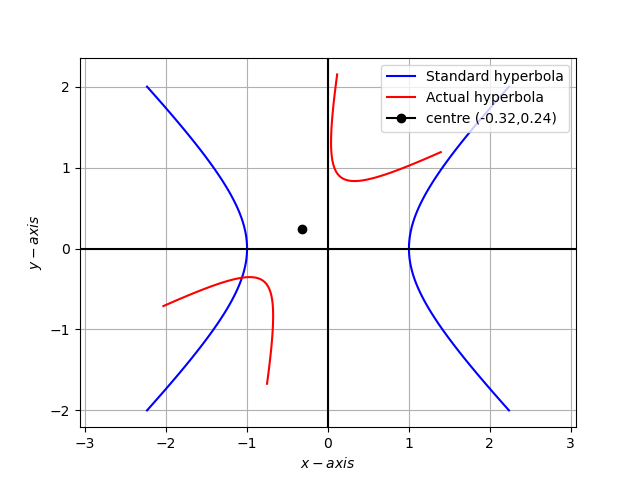
\includegraphics[width=\columnwidth]{./figs/hyperbola_2.png}
\caption{Comparison of the Standerd and Actual Hyperbola}
\label{fig:hyperbola}
\end{figure}
\renewcommand{\theequation}{\theenumi}
\begin{enumerate}[label=\thesection.\arabic*.,ref=\thesection.\theenumi]
\numberwithin{equation}{enumi}
\item Verification of the above problem using python code.\\
\solution The  following Python code generates Fig. \ref{fig:hyperbola}
\begin{lstlisting}
codes/hyperbola_3.py
\end{lstlisting}
%
\end{enumerate}

\end{document}



